\documentclass{article}

\usepackage{fullpage}
\usepackage{url}
\usepackage{bbm}
\usepackage{graphicx}
\usepackage{amsmath}
\usepackage{physics}
\usepackage{mathtools}
\usepackage{bbold}
\usepackage{slashed}
\usepackage{pxfonts}
\usepackage{multicol}
\usepackage{mathptmx}
\usepackage{simplewick}
\usepackage{placeins}
\usepackage{tikz}
\usepackage{tikz-feynman}

\usepackage{lmodern}
\usepackage[T1]{fontenc}
\usepackage[fontsize=13.5pt]{fontsize}

\DeclareMathOperator{\erfi}{erfi}
\newcommand{\R}{\ensuremath{\mathbb{R}}}
\newcommand{\C}{\ensuremath{\mathbb{C}}}

\title{Quantum Field Theory I Excercise 8}
\author{Idan Stark}
\date{\today}

\begin{document}
\maketitle

\section{A different gauge fixing}
In class we used the gauge fixing
\begin{equation}
    G[A] = \partial_\mu A^\mu - \omega(x) = 0
\end{equation}
Instead, in this section, we use:
\begin{equation}
    G[A] = A_0 - \omega(x) = 0
\end{equation}

\subsection{The path integral form}
Starting from the generic form, using the fact that for an Abelian gauage theory the determinant is independent of $\alpha = \omega(x)$:
\begin{equation}
    Z = \det(-\frac{1}{e}\partial^2) \int \mathcal{D}A_\mu e^{iS[A]}\delta(A_0 - \omega(x))
\end{equation}
And then integrating with respect to $\omega(x)$ abd applying the same gaussian weight:
\begin{equation}
    \int \mathcal{D} \omega(x) e^{i \int \frac{\omega^2}{2\xi} d^4x} Z = \det(-\frac{1}{e}\partial^2)\int \mathcal{D} \omega(x) e^{i \int \frac{\omega^2}{2\xi} d^4x} \int \mathcal{D}A_\mu e^{iS[A]}\delta(A_0 - \omega(x))
\end{equation}
Using the delta function for the $\omega$ integral on the RHS and renaming the LHS integral which is a constant:
\begin{equation}
    Z = C \int \mathcal{D} A_\mu e^{iS[A] - i \int d^4x \frac{A_0^2}{2\xi}}
\end{equation}
\subsection{The photon propegator}
Similar to the gauge fixing we did in class, we can now find the propegator using the inverse to the quadratic term in the action. The action in momentum space:
\begin{equation}
\begin{gathered}
    \tilde{S} = \frac{1}{2} \int \frac{d^4k}{(2\pi)^4}\tilde{A}_\mu(k) (-k^2 \eta^{\mu\nu} + k^\mu k^\nu)\tilde{A}_\nu - \frac{1}{\xi^2}\tilde{A}_0^2 = \\ =
    \frac{1}{2} \int \frac{d^4k}{(2\pi)^4}\tilde{A}_\mu(k)0\left(-k^2 \eta^{\mu\nu} + k^\mu k^\nu - \frac{1}{\xi^2}u^{\mu}u^{\nu}\right)\tilde{A}_\nu
\end{gathered}
\end{equation}
Where we defined $u^\mu = \eta^{\mu0} = (1, \vec{0})$. We can invert the matrix:
\begin{equation}
    \left(-k^2 \eta^{\mu\nu} + k^\mu k^\nu - \frac{1}{\xi^2}u^{\mu}u^{\nu}\right) \tilde{D}_F^{\nu\rho}(k) = i\delta^\rho_\nu
\end{equation}
Similar to the propegator we found in class, we will look for a matrix with a similar structure to the original:
\begin{equation}
    \tilde{D}_F^{\mu\nu}(k) = -\frac{i}{k^2} \left(\eta^{\mu\nu} + A k^{\mu}k^{\nu} + B u^{\mu}u^{\nu} + C(k^{\mu}u^{\nu} + u^{\mu}k^{\nu})\right)
\end{equation}
Where we included all terms that are invariant under 3d rotations. Plugging this in gives:
\begin{equation}
    \left(-k^2 \eta^{\mu\nu} + k^\mu k^\nu - \frac{1}{\xi^2}u^{\mu}u^{\nu}\right) \frac{-i}{k^2} \left(\eta^{\nu\rho} + A k^{\nu}k^{\rho} + B u^{\nu}u^{\rho} + C(k^{\nu}u^{\rho} + u^{\nu}k^{\rho})\right) = i\delta^\rho_\mu
\end{equation}
\begin{equation}
    \left(\eta^{\mu\nu} - \frac{k^\mu k^\nu}{k^2} + \frac{1}{k^2\xi^2}u^{\mu}u^{\nu}\right) \left(\eta^{\nu\rho} + A k^{\nu}k^{\rho} + B u^{\nu}u^{\rho} + C(k^{\nu}u^{\rho} + u^{\nu}k^{\rho})\right) = \delta^\rho_\mu
\end{equation}
\begin{equation}
\begin{gathered}
    \delta^{\rho}_{\mu} + A k^{\mu}k^{\rho} + B u^{\mu}u^{\rho} + C(k^{\mu}u^{\rho} + u^{\mu}k^{\rho}) - \\ -
    \frac{k^\mu k^\rho}{k^2} - Ak^\mu k^\rho - B \frac{k\cdot u}{k^2} k^\mu u^\rho - C \left(k^\mu u^{\rho} + \frac{k\cdot u}{k^2} k^{\mu}k^{\rho}\right) + \\ +
    \frac{1}{k^2\xi^2}u^{\mu}u^{\rho} + A \frac{k\cdot u}{k^2\xi^2} u^{\mu}k^{\rho} + B \frac{1}{k^2\xi^2} u^{\mu}u^{\rho} + C\left(\frac{k\cdot u}{k^2\xi^2}u^{\mu}u^{\rho} + \frac{1}{k^2\xi^2}u^{\mu}k^{\rho}\right) = \delta^\rho_\mu
\end{gathered}
\end{equation}
Gathering similar terms:
\begin{equation}
\begin{gathered}
    \left(B + \frac{1}{k^2\xi^2} + B \frac{1}{k^2\xi^2} + C \frac{k\cdot u}{k^2\xi^2}\right)u^\mu u^\rho
    - \\ -
    \left(C \frac{k\cdot u}{k^2} + \frac{1}{k^2}\right) k^\mu k^\rho
    - \\ -
    B \frac{k\cdot u}{k^2} k^\mu u^\rho
    + \\ +
    \left(C + A \frac{k\cdot u}{k^2\xi^2} + C \frac{1}{k^2\xi^2}\right) u^\mu k^\rho
    = 0
\end{gathered}
\end{equation}
By requiring all terms to cancel we get:
\begin{equation}
    A = \frac{1 + k^2\xi^2}{(k\cdot u)^2}
    \qquad
    B = 0
    \qquad
    C = -\frac{1}{k\cdot u}
\end{equation}
So, the final propegator is:
\begin{equation}
    D_F^{\mu\nu} = -\frac{i}{k^2 + i\epsilon} \left(\eta^{\mu\nu} + \frac{1 + k^2\xi^2}{(k\cdot u)^2} k^{\mu}k^{\nu} - \frac{1}{k\cdot u} (k^{\mu}u^{\nu} + u^{\mu}k^{\nu})\right)
\end{equation}
Or, for simplicity, setting $\xi^2 = 0$:
\begin{equation}
    D_F^{\mu\nu} = -\frac{i}{k^2 + i\epsilon} \left(\eta^{\mu\nu} + \frac{1}{(k\cdot u)^2} k^{\mu}k^{\nu} - \frac{1}{k\cdot u} (k^{\mu}u^{\nu} + u^{\mu}k^{\nu})\right)
\end{equation}
\subsection{Comparing scattering amplitudes}
Let us now calculate the physical correlation function $\langle F_{\mu\nu} F_{\rho\sigma} \rangle$ in both gauages. To do that, we express it using the field $A^{\mu}$:
\begin{equation}
    F_{\mu\nu} = \partial_\mu A_\nu - \partial_\nu A_\mu
\end{equation}
\begin{equation}
\begin{gathered}
    F_{\mu\nu} F_{\rho\sigma} =
    \left(\partial_\mu A_\nu - \partial_\nu A_\mu\right)
    \left(\partial_\rho A_\sigma - \partial_\sigma A_\rho\right) = \\ =
    \partial_\mu A_\nu \partial_\rho A_\sigma - \partial_\nu A_\mu \partial_\rho A_\sigma -
    \partial_\mu A_\nu \partial_\sigma A_\rho + \partial_\nu A_\mu \partial_\sigma A_\rho
\end{gathered}
\end{equation}
Going to momentum space $A_\mu(x) \rightarrow \tilde{A}_\mu(k)$ gives:
\begin{equation}
\begin{gathered}
    \langle \tilde{F}_{\mu\nu}(k) \tilde{F}_{\rho\sigma}(-k) \rangle = \\ =
    -\langle k_\mu A_\nu(k) k'_\rho A_\sigma(-k) \rangle + \langle k_\nu A_\mu(k) k_\rho A_\sigma(-k) \rangle + \\ +
    \langle k_\mu A_\nu(k) k_\sigma A_\rho(-k) \rangle - \langle k_\nu A_\mu(k) k_\sigma A_\rho(-k) \rangle = \\ =
    - k_\mu k_\rho \langle A_\nu(k) A_\sigma(-k) \rangle + k_\nu k_\rho \langle A_\mu(k) A_\sigma(-k) \rangle + \\ +
    k_\mu k_\sigma \langle A_\nu(k) A_\rho(-k) \rangle - k_\nu k_\sigma \langle A_\mu(k) A_\rho(-k) \rangle
\end{gathered}
\end{equation}
Using the gauage we found in class:
\begin{equation}
    \langle A_\mu(k) A_\nu (-k) \rangle = \frac{- i \eta^{\mu\nu}}{k^2 + i\epsilon}
\end{equation}
This becomes:
\begin{equation}
\begin{gathered}
    \langle \tilde{F}_{\mu\nu}(k) \tilde{F}_{\rho\sigma}(-k) \rangle =
    k_\mu k_\rho \frac{i \eta^{\nu\sigma}}{k^2 + i\epsilon} - k_\nu k_\rho  \frac{i \eta^{\mu\sigma}}{k^2 + i\epsilon} -
    k_\mu k_\sigma \frac{i \eta^{\nu\rho}}{k^2 + i\epsilon} + k_\nu k_\sigma  \frac{i \eta^{\mu\rho}}{k^2 + i\epsilon} = \\ =
    \frac{i}{k^2 + i\epsilon} \left[
        k_\mu k_\rho \eta^{\nu\sigma} - 
        k_\nu k_\rho \eta^{\mu\sigma} - 
        k_\mu k_\sigma \eta^{\nu\rho} + 
        k_\nu k_\sigma \eta^{\mu\rho}
    \right]
\end{gathered}
\end{equation}
In our new gauge:
\begin{equation}
    \langle A_\mu(k) A_\nu (-k) \rangle = -\frac{i}{k^2 + i\epsilon} \left(\eta^{\mu\nu} + \frac{1}{(k\cdot u)^2} k^{\mu}k^{\nu} - \frac{1}{k\cdot u} (k^{\mu}u^{\nu} + u^{\mu}k^{\nu})\right)
\end{equation}
Which gives:
\begin{equation}
\begin{gathered}
    \langle \tilde{F}_{\mu\nu}(k) \tilde{F}_{\rho\sigma}(-k) \rangle =
    \frac{i}{k^2 + i\epsilon} \Big[
        k_\mu k_\rho \eta^{\nu\sigma} - 
        k_\nu k_\rho \eta^{\mu\sigma} - 
        k_\mu k_\sigma \eta^{\nu\rho} + 
        k_\nu k_\sigma \eta^{\mu\rho} + \\ +
        \frac{1}{(k\cdot u)^2} \left[
            k_\mu k_\rho k_\nu k_\sigma - 
            k_\nu k_\rho k_\mu k_\sigma - 
            k_\mu k_\sigma k_\nu k_\rho + 
            k_\nu k_\sigma k_\mu k_\rho
        \right] + \\ +
        \frac{1}{k\cdot u} \left[
            k_\mu k_\rho k_\nu u_\sigma - 
            k_\nu k_\rho k_\mu u_\sigma - 
            k_\mu k_\sigma k_\nu u_\rho + 
            k_\nu k_\sigma k_\mu u_\rho
        \right] + \\ +
        \frac{1}{k\cdot u} \left[
            k_\mu k_\rho u_\nu k_\sigma - 
            k_\nu k_\rho u_\mu k_\sigma - 
            k_\mu k_\sigma u_\nu k_\rho + 
            k_\nu k_\sigma u_\mu k_\rho
        \right]
    \Big] = \\ =
    \frac{i}{k^2 + i\epsilon} \left[
        k_\mu k_\rho \eta^{\nu\sigma} - 
        k_\nu k_\rho \eta^{\mu\sigma} - 
        k_\mu k_\sigma \eta^{\nu\rho} + 
        k_\nu k_\sigma \eta^{\mu\rho}
    \right]
\end{gathered}
\end{equation}
Where in the last line most of the terms canceled. This result is exactly the same as the result from the gauge we used in class.

\newpage
\section{Constraints from charge conjugation}
\subsection{one-photon correlation function}
In first loop order, the two diagrams that contribute to the 1PI correlation function are the 1 point loop in either clockwise or counter-clockwise directions. This diagram has a single vertex, a single internal fermion propegator, and a single external photon propegator:
\begin{equation}
    \langle A_\mu(p_1) \rangle = (-ie)\frac{-i\eta_{\mu\nu}}{p_1^2 + i\epsilon}\int \frac{d^4k}{(2\pi)^4}\Tr[\frac{i\gamma^\nu \left(\slashed{k} + m\right)}{k^2 - m^2 + i\epsilon}]
\end{equation}
The trace inside the integral has two terms, one proportional to a single gamma matric, and one to the product of two gamma matrices. Using the identities:
\begin{equation}
    \Tr[\gamma^\mu] = 0
    \qquad
    \Tr[\gamma^\mu\gamma^\nu] = 4\eta^{\mu\nu}
\end{equation}
We get:
\begin{equation}
    \langle A_\mu \rangle \propto \eta_{\mu\nu} \eta^{\nu\alpha} \int \frac{d^4k}{(2\pi)^4}\frac{k_\alpha}{k^2 - m^2 + i\epsilon}
\end{equation}
Finally, using
\begin{equation}
    \eta_{\mu\nu} \eta^{\mu\alpha} = \delta_\nu^\alpha
\end{equation}
We get:
\begin{equation}
    \langle A_\mu \rangle \propto \int \frac{d^4k}{(2\pi)^4}\frac{k_\mu}{k^2 - m^2 + i\epsilon}
\end{equation}
This integrand has an even measure and an odd integrand, and so it vanished:
\begin{equation}
    \langle A_\mu \rangle = 0
\end{equation}
\subsection{three-photons correlation function}
Now, let us look at the three photon correlation function. This function has the exact same structure: one loop, only this time with three internal fermion propegators, three external photon propegators, and three vertices. The overall contribution from each of the diagrams (one clockwise and one counter-clockwise), is again proportional to the integral over the internal momentum $k$:
\begin{equation}
\begin{gathered}
    \langle A_\mu(p_1) A_\nu(p_2) A_\rho(p_3) \rangle \propto
    D_{\mu\alpha}(p_1)
    D_{\nu\beta}(p_2)
    D_{\rho\gamma}(p_3)
    \times \\ \times
    \int \frac{d^4k}{(2\pi)^4}
    \Tr[
        \gamma^\alpha S_F(k + p_1)
        \gamma^\beta S_F(k + p_1 + p_2)
        \gamma^\gamma S_F(k)
    ]
\end{gathered}
\end{equation}
The important difference between the clockwise and counter-clockwise diagrams is in the order of matrix multiplication. This can be seen in figure 1.
\begin{figure}[ht]
    \centering

    \begin{minipage}{0.48\textwidth}
        \centering
        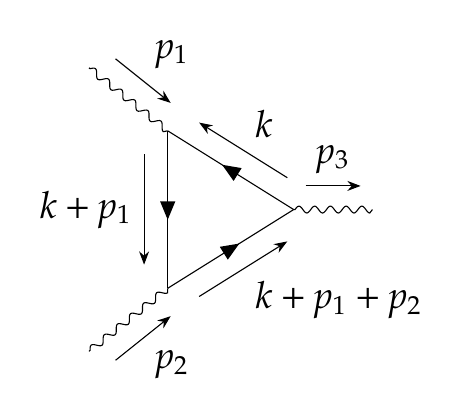
\begin{tikzpicture}
        \begin{feynman}
            \vertex (a) at (-0.6,1);
            \vertex (b) at (-0.6,-1);
            \vertex (c) at (1,0);

            \draw[fermion, momentum'=$k + p_1$] (a) -- (b);
            \draw[fermion, momentum'=$k + p_1 + p_2$] (b) -- (c);
            \draw[fermion, momentum'=$k$] (c) -- (a);

            \draw[photon, momentum=$p_1$] (-1.6,1.8) -- (a);
            \draw[photon, momentum'=$p_2$] (-1.6,-1.8) -- (b);
            \draw[photon, momentum=$p_3$] (c) -- +(1,0);
        \end{feynman}
        \end{tikzpicture}
    \end{minipage}
    \hfill
    \begin{minipage}{0.48\textwidth}
        \centering
        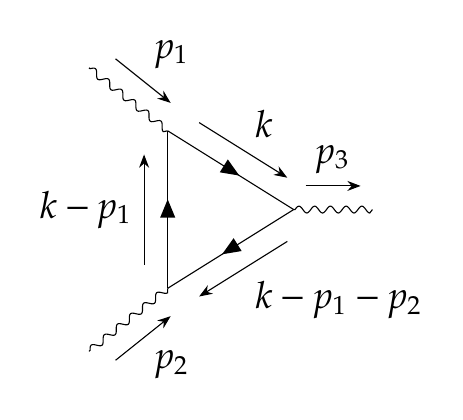
\begin{tikzpicture}
        \begin{feynman}
            \vertex (a) at (-0.6,1);
            \vertex (b) at (-0.6,-1);
            \vertex (c) at (1,0);

            \draw[fermion, momentum=$k - p_1$] (b) -- (a);
            \draw[fermion, momentum=$k - p_1 - p_2$] (c) -- (b);
            \draw[fermion, momentum=$k$] (a) -- (c);

            \draw[photon, momentum=$p_1$] (-1.6,1.8) -- (a);
            \draw[photon, momentum'=$p_2$] (-1.6,-1.8) -- (b);
            \draw[photon, momentum=$p_3$] (c) -- +(1,0);
        \end{feynman}
        \end{tikzpicture}
    \end{minipage}

    \caption{The two options for the one loop 3 photon diagram, on the left tis the clockwise and on the right is the counter-clockwise.}
    \label{fig:threephoton}
\end{figure}

This means that the trace in the counter-clockwise diagrams is:
\begin{equation}
    \Tr[
        \gamma^\alpha S_F(k)
        \gamma^\gamma S_F(k - p_1 - p_2)
        \gamma^\beta S_F(k - p_1)
    ]
\end{equation}
Under chareg conjugation, gamma matrices tranform according to Clifford algebra, while the fermion propegators transform by changing the sign of their momentum and transposing:
\begin{equation}
    C \gamma^{\mu} C^T = -\gamma^{\mu T}
    \qquad
    C S_F(k) C^T = S_F^T(-k)
\end{equation}
So:
\begin{equation}
\begin{gathered}
    \Tr[
        \gamma^\alpha S_F(k) \gamma^\gamma S_F(k - p_1 - p_2) \gamma^\beta S_F(k - p_1)
    ] = \\ =
    \Tr[
        \gamma^\alpha C^T C S_F(k) C^T C \gamma^\gamma C^T C S_F(k - p_1 - p_2) C^T C \gamma^\beta C^T C S_F(k - p_1) C^T C 
    ] = \\ =
    \Tr[
        C \gamma^\alpha C^T C S_F(k) C^T C \gamma^\gamma C^T C S_F(k - p_1 - p_2) C^T C \gamma^\beta C^T C S_F(k - p_1) C^T
    ] = \\ =
    (-1)^3\Tr[
        \gamma^{\alpha T} S_F^T(-k) \gamma^{\gamma T} S_F^T(- k + p_1 + p_2) \gamma^{\beta T} S_F^T(- k + p_1)
    ]
\end{gathered}
\end{equation}
Changing integration variable $k \rightarrow -k$:
\begin{equation}
\begin{gathered}
    -\Tr[
        \gamma^{\alpha T} S_F^T(k) \gamma^{\gamma T} S_F^T(k + p_1 + p_2) \gamma^{\beta T} S_F^T(k + p_1)
    ] = \\ =
    -\Tr[
        S_F(k + p_1)
        \gamma^{\beta}
        S_F(k + p_1 + p_2)
        \gamma^{\gamma}
        S_F(k)
        \gamma^{\alpha}
    ] = \\ =
    -\Tr[
        \gamma^{\alpha}
        S_F(k + p_1)
        \gamma^{\beta}
        S_F(k + p_1 + p_2)
        \gamma^{\gamma}
        S_F(k)
    ]
\end{gathered}
\end{equation}
Which means that this diagram is the exact opposite of the clockwise diagram, and thus their sum contribution is zero.
\newpage
\section{Examples of the Ward-Takahashi identity}
\subsection{The scattering amplitude in Compton scattering}
The scattering amplitude in Compton scattering is:
\begin{equation}
\begin{gathered}
    i\mathcal{M} =
    \bar{u}(p')(-ie\gamma^\mu)\epsilon_\mu^*(k') \frac{i(\slashed{p} + \slashed{k} + m)}{(p + k)^2 - m^2 + i\epsilon}(-ie\gamma^\nu)\epsilon_\nu(k)u(p) + \\ +
    \bar{u}(p')(-ie\gamma^\nu)\epsilon_\nu^*(k) \frac{i(\slashed{p} - \slashed{k}' + m)}{(p - k')^2 - m^2 + i\epsilon}(-ie\gamma^\mu)\epsilon_\mu(k')u(p)
\end{gathered}
\end{equation}
Setting each photon polarization to be parallel to its momentum $\epsilon_\mu(k) \propto k_\mu$ gives:
\begin{equation}
\begin{gathered}
    i\mathcal{M} \propto
    \bar{u}(p')(-ie\gamma^\mu)k'_\mu \frac{i(\slashed{p} + \slashed{k} + m)}{(p + k)^2 - m^2 + i\epsilon}(-ie\gamma^\nu)k_\nu u(p) + \\ +
    \bar{u}(p')(-ie\gamma^\nu)k_\nu \frac{i(\slashed{p} - \slashed{k}' + m)}{(p - k')^2 - m^2 + i\epsilon}(-ie\gamma^\mu)k'_\mu u(p)
\end{gathered}
\end{equation}
As we saw in class:
\begin{equation}
    (p + k)^2 - m^2 = 2p\cdot k \qquad (p - k')^2 - m^2 = -2p\cdot k'
\end{equation}
So:
\begin{equation}
\begin{gathered}
    i\mathcal{M} \propto
    \bar{u}(p') \left[
        \slashed{k}' \frac{\slashed{p} + \slashed{k} + m}{2p\cdot k + i\epsilon}\slashed{k} -
        \slashed{k} \frac{\slashed{p} - \slashed{k}' + m}{2p\cdot k' + i\epsilon}\slashed{k}'
    \right] u(p)
\end{gathered}
\end{equation}
Now, looking at the brackets, there are three interesting pairs of terms matching in the two fractions. The second pair is proportional to the photon mass, so it vanishes:
\begin{equation}
    \frac{\slashed{k}'\slashed{k}\slashed{k}}{2p\cdot k} + \frac{\slashed{k}\slashed{k}'\slashed{k}'}{2p\cdot k'} = \frac{\slashed{k}'k^2}{2p\cdot k} + \frac{\slashed{k}k'^2}{2p\cdot k'} = 0
\end{equation}
The other two terms match another identity we saw in class:
\begin{equation}
    \left(\slashed{p} + m\right)\gamma^\mu u(p) = 2p^\mu u(p)
\end{equation}
And similarly, the same will work from the left:
\begin{equation}
\begin{gathered}
    \bar{u}(p) \gamma^\mu \left(\slashed{p} + m\right) =
    \bar{u}(p) \left(\gamma^\mu \gamma^\nu p_\nu + \gamma^\mu m\right) = \\ =
    \bar{u}(p) \left(2 p^\mu - \slashed{p}\gamma^\mu + m \gamma^\mu\right) =
    2 \bar{u}(p) p^\mu - \bar{u}(p) \left(\slashed{p} + m \right)\gamma^\mu =
    2 \bar{u}(p) p^\mu
\end{gathered}
\end{equation}
We want to apply the first identity for the first term in the brackets and the second identity for the second term in the brackets, so that we are left with the same $k$ dependence in both terms. This requires the second term to have $p'$ and not $p$ in the nominator. So, we use conservation of momentum:
\begin{equation}
\begin{gathered}
    p - k' = p' - k
    \\
    p\cdot k' = -\frac{1}{2}\left[(p - k')^2 - m^2\right] = -\frac{1}{2}\left[(p' - k)^2 - m^2\right] = p' \cdot k
\end{gathered}
\end{equation}
So we can rewrite:
\begin{equation}
    i\mathcal{M} \propto
    \bar{u}(p') \left[
        \slashed{k}' \frac{\slashed{p} + m}{2p\cdot k + i\epsilon}\slashed{k} -
        \slashed{k} \frac{\slashed{p}' + m}{2p'\cdot k + i\epsilon}\slashed{k}'
    \right] u(p)
\end{equation}
\begin{equation}
    i\mathcal{M} \propto
    \bar{u}(p') \left[
        \slashed{k}' \frac{p\cdot k}{p\cdot k + i\epsilon} -
        \frac{p' \cdot k}{p'\cdot k + i\epsilon}\slashed{k}'
    \right] u(p)
\end{equation}
\begin{equation}
    i\mathcal{M} \propto
    \bar{u}(p') \left[
        \slashed{k}' -
        \slashed{k}'
    \right] u(p) = 0
\end{equation}
\subsection{No counter terms in the 4-photon scattering}
There are six diagrams in the 4-photon scattering, matching the three possible topology of the photons, with two directions of the loop in each topology:
\begin{figure}[ht]
    \centering

    \begin{minipage}{0.31\textwidth}
        \centering
        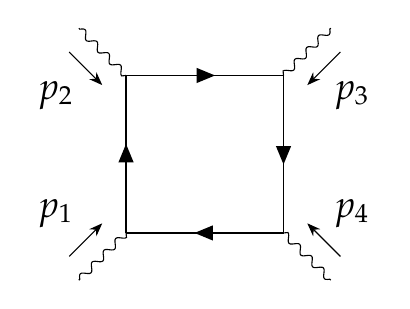
\begin{tikzpicture}
        \begin{feynman}
            \vertex (a) at (-1,-1);
            \vertex (b) at (-1,1);
            \vertex (c) at (1,-1);
            \vertex (d) at (1,1);

            \draw[fermion] (a) -- (b);
            \draw[fermion] (b) -- (d);
            \draw[fermion] (d) -- (c);
            \draw[fermion] (c) -- (a);

            \draw[photon, momentum=$p_1$] (-1.6,-1.6) -- (a);
            \draw[photon, momentum'=$p_2$] (-1.6,1.6) -- (b);
            \draw[photon, momentum'=$p_4$] (1.6,-1.6) -- (c);
            \draw[photon, momentum=$p_3$] (1.6,1.6) -- (d);
        \end{feynman}
        \end{tikzpicture}
    \end{minipage}
    \hfill
    \begin{minipage}{0.31\textwidth}
        \centering
        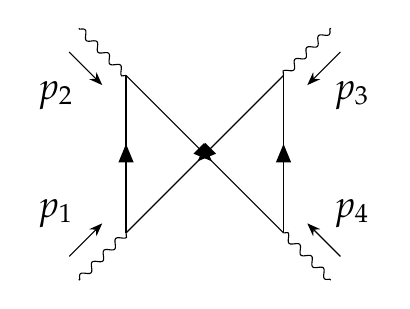
\begin{tikzpicture}
        \begin{feynman}
            \vertex (a) at (-1,-1);
            \vertex (b) at (-1,1);
            \vertex (c) at (1,-1);
            \vertex (d) at (1,1);

            \draw[fermion] (a) -- (b);
            \draw[fermion] (b) -- (c);
            \draw[fermion] (c) -- (d);
            \draw[fermion] (d) -- (a);

            \draw[photon, momentum=$p_1$] (-1.6,-1.6) -- (a);
            \draw[photon, momentum'=$p_2$] (-1.6,1.6) -- (b);
            \draw[photon, momentum'=$p_4$] (1.6,-1.6) -- (c);
            \draw[photon, momentum=$p_3$] (1.6,1.6) -- (d);
        \end{feynman}
        \end{tikzpicture}
    \end{minipage}
    \begin{minipage}{0.31\textwidth}
        \centering
        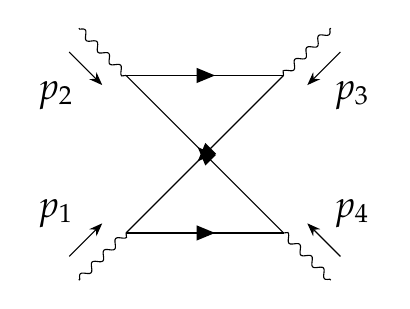
\begin{tikzpicture}
        \begin{feynman}
            \vertex (a) at (-1,-1);
            \vertex (b) at (-1,1);
            \vertex (c) at (1,-1);
            \vertex (d) at (1,1);

            \draw[fermion] (a) -- (c);
            \draw[fermion] (c) -- (b);
            \draw[fermion] (b) -- (d);
            \draw[fermion] (d) -- (a);

            \draw[photon, momentum=$p_1$] (-1.6,-1.6) -- (a);
            \draw[photon, momentum'=$p_2$] (-1.6,1.6) -- (b);
            \draw[photon, momentum'=$p_4$] (1.6,-1.6) -- (c);
            \draw[photon, momentum=$p_3$] (1.6,1.6) -- (d);
        \end{feynman}
        \end{tikzpicture}
    \end{minipage}
    \begin{minipage}{0.31\textwidth}
        \centering
        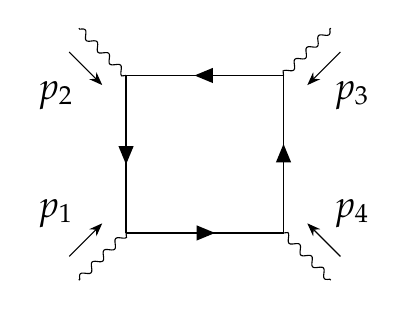
\begin{tikzpicture}
        \begin{feynman}
            \vertex (a) at (-1,-1);
            \vertex (b) at (-1,1);
            \vertex (c) at (1,-1);
            \vertex (d) at (1,1);

            \draw[fermion] (b) -- (a);
            \draw[fermion] (d) -- (b);
            \draw[fermion] (c) -- (d);
            \draw[fermion] (a) -- (c);

            \draw[photon, momentum=$p_1$] (-1.6,-1.6) -- (a);
            \draw[photon, momentum'=$p_2$] (-1.6,1.6) -- (b);
            \draw[photon, momentum'=$p_4$] (1.6,-1.6) -- (c);
            \draw[photon, momentum=$p_3$] (1.6,1.6) -- (d);
        \end{feynman}
        \end{tikzpicture}
    \end{minipage}
    \hfill
    \begin{minipage}{0.31\textwidth}
        \centering
        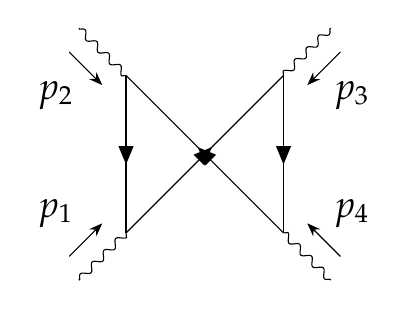
\begin{tikzpicture}
        \begin{feynman}
            \vertex (a) at (-1,-1);
            \vertex (b) at (-1,1);
            \vertex (c) at (1,-1);
            \vertex (d) at (1,1);

            \draw[fermion] (b) -- (a);
            \draw[fermion] (c) -- (b);
            \draw[fermion] (d) -- (c);
            \draw[fermion] (a) -- (d);

            \draw[photon, momentum=$p_1$] (-1.6,-1.6) -- (a);
            \draw[photon, momentum'=$p_2$] (-1.6,1.6) -- (b);
            \draw[photon, momentum'=$p_4$] (1.6,-1.6) -- (c);
            \draw[photon, momentum=$p_3$] (1.6,1.6) -- (d);
        \end{feynman}
        \end{tikzpicture}
    \end{minipage}
    \begin{minipage}{0.31\textwidth}
        \centering
        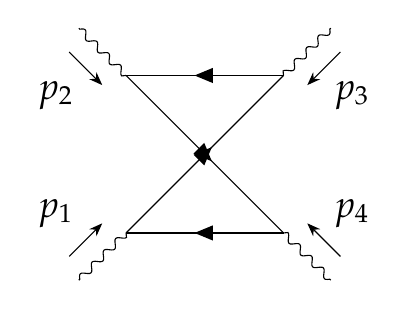
\begin{tikzpicture}
        \begin{feynman}
            \vertex (a) at (-1,-1);
            \vertex (b) at (-1,1);
            \vertex (c) at (1,-1);
            \vertex (d) at (1,1);

            \draw[fermion] (c) -- (a);
            \draw[fermion] (b) -- (c);
            \draw[fermion] (d) -- (b);
            \draw[fermion] (a) -- (d);

            \draw[photon, momentum=$p_1$] (-1.6,-1.6) -- (a);
            \draw[photon, momentum'=$p_2$] (-1.6,1.6) -- (b);
            \draw[photon, momentum'=$p_4$] (1.6,-1.6) -- (c);
            \draw[photon, momentum=$p_3$] (1.6,1.6) -- (d);
        \end{feynman}
        \end{tikzpicture}
    \end{minipage}

    \caption{The six diagrams for the four photons correlation function in one loop order.}
    \label{fig:fourphoton}
\end{figure}
The contribution from the first diagram is (with the spinor indices $\mu, \nu\, \sigma, \rho$ matching the photon momenta $p_1, p_2, p_3, p_4$, which are all incoming, starting from the propegator going into the vertex with $p_1$):
\begin{equation}
\begin{gathered}
    i \mathcal{M}_1 =
    -(-ie)^4\epsilon^*_\sigma(p_3)\epsilon^*_\rho(p_4)
    \int \frac{d^4k}{(2\pi)^4}
    \times \\ \times
    \Tr[S_F(k)\gamma^\mu S_F(k + p_1) \gamma^\nu S_F(k + p_1 + p_2)\gamma^\sigma S_F(k + p_1 + p_2 + p_3) \gamma^\rho]
    \times \\ \times
    \epsilon_\mu(p_1)\epsilon_\nu(p_2)
\end{gathered}
\end{equation}
Each propegator is quadratic in $k$ in the denominator and has a term in the nominator that is linear in $k$ plus a constant. The logarithmically divergent part is the product of all linar parts in the nominators, since then the integral is of order $d^4k \left(\frac{k}{k^2}\right)^4 \sim k^{-1} dk$. In this diagram, this gives:
\begin{equation}
\begin{gathered}
    i \mathcal{M}_1 \supset
    -(-ie)^4\epsilon^*_\sigma(p_3)\epsilon^*_\rho(p_4)
    \int \frac{d^4k}{(2\pi)^4}
    \times \\ \times
    \Tr\Big[\frac{\slashed{k}}{k^2 - m^2 + i\epsilon}\gamma^\mu \frac{\slashed{k}}{(k + p_1)^2 - m^2 + i\epsilon}
    \times \\ \times
    \gamma^\nu\frac{\slashed{k}}{(k + p_1 + p_2)^2 - m^2 + i\epsilon}\gamma^\sigma \frac{\slashed{k}}{(k + p_1 + p_2 + p_3)^2 - m^2 + i\epsilon}\gamma^\rho \Big]
    \times \\ \times
    \epsilon_\mu(p_1)\epsilon_\nu(p_2)
\end{gathered}
\end{equation}
The contribution from the matching counter-clockwise diagram will be the same, but the momenta are reversed (techinqually the order of the matrices in the loop is also reversed, but since for an even number of gamma matrices the order in the trace can be flipped without change of sign, we can ignore that):
\begin{equation}
\begin{gathered}
    i \mathcal{M}_1^{cc} \supset
    -(-ie)^4\epsilon^*_\sigma(p_3)\epsilon^*_\rho(p_4)
    \int \frac{d^4k}{(2\pi)^4}
    \times \\ \times
    \Tr\Big[\frac{\slashed{k}}{k^2 - m^2 + i\epsilon}\gamma^\mu \frac{\slashed{k}}{(k - p_1)^2 - m^2 + i\epsilon}
    \times \\ \times
    \gamma^\nu\frac{\slashed{k}}{(k - p_1 - p_2)^2 - m^2 + i\epsilon}\gamma^\sigma \frac{\slashed{k}}{(k - p_1 - p_2 - p_3)^2 - m^2 + i\epsilon}\gamma^\rho \Big]
    \times \\ \times
    \epsilon_\mu(p_1)\epsilon_\nu(p_2)
\end{gathered}
\end{equation}
Changing variables $k \rightarrow -k$ results in the same contribution as the one for the clockwise loop. This is a general result, and so we can sum only the three clockwise loops. Now, in the short distance (high energy) limit where $k^2 \gg m^2$, the fermion momenta and the fermion mass in the denominator are negligable, and the diagram becomes:
\begin{equation}
\begin{gathered}
    i \mathcal{M}_1 \supset
    -(-ie)^4\epsilon^*_\sigma(p_3)\epsilon^*_\rho(p_4)
    \int \frac{d^4k}{(2\pi)^4}
    \times \\ \times
    \Tr\Big[\frac{\slashed{k}}{k^2 + i\epsilon}\gamma^\mu \frac{\slashed{k}}{k^2 + i\epsilon}
    \gamma^\nu\frac{\slashed{k}}{k^2 + i\epsilon}\gamma^\sigma \frac{\slashed{k}}{k^2 + i\epsilon}\gamma^\rho \Big]
    \epsilon_\mu(p_1)\epsilon_\nu(p_2)
\end{gathered}
\end{equation}
We can then pull all the denominator scalars out of the trace to get:
\begin{equation}
\begin{gathered}
    i \mathcal{M}_1 \supset
    -(-ie)^4\epsilon^*_\sigma(p_3)\epsilon^*_\rho(p_4)
    \int \frac{d^4k}{(2\pi)^4} \frac{1}{k^8}
    \times \\ \times
    \Tr[\slashed{k}\gamma^\mu \slashed{k}
    \gamma^\nu\slashed{k} \gamma^\sigma \slashed{k} \gamma^\rho]
    \epsilon_\mu(p_1)\epsilon_\nu(p_2)
\end{gathered}
\end{equation}
So, the only remaining difference between the three clockwise diagrams are the traces. The three traces from the three clockwise diagrams are:
\begin{equation}
\begin{gathered}
    \Tr[
        \slashed{k}\gamma^\mu
        \slashed{k}\gamma^\nu
        \slashed{k}\gamma^\sigma
        \slashed{k}\gamma^\rho
    ]
    \\
    \Tr[
        \slashed{k}\gamma^\mu
        \slashed{k}\gamma^\nu
        \slashed{k}\gamma^\rho
        \slashed{k}\gamma^\sigma
    ]
    \\
    \Tr[
        \slashed{k}\gamma^\mu
        \slashed{k}\gamma^\rho
        \slashed{k}\gamma^\nu
        \slashed{k}\gamma^\sigma
    ]
\end{gathered}
\end{equation}
Now, let us use:
\begin{equation}
    \slashed{k}\gamma^\mu = k_\alpha \gamma^\alpha \gamma^\mu = k_\alpha \left(2 \eta^{\alpha\mu} - \gamma^\mu \gamma^\alpha\right) = 
    2 k^\mu - \gamma^\mu \slashed{k}
\end{equation}
Using this for two of the four indices, the sum of the three traces becomes:
\begin{equation}
\begin{gathered}
    \Tr \Big[
    \slashed{k}\gamma^\mu
    \slashed{k}\gamma^\nu
    \slashed{k}\gamma^\sigma
    \slashed{k}\gamma^\rho +
    \slashed{k}\gamma^\mu
    \slashed{k}\gamma^\nu
    \slashed{k}\gamma^\rho
    \slashed{k}\gamma^\sigma +
    \slashed{k}\gamma^\mu
    \slashed{k}\gamma^\rho
    \slashed{k}\gamma^\nu
    \slashed{k}\gamma^\sigma \Big] = \\ =
    \Tr \Big[
    \slashed{k}\gamma^\mu
    \left(2 k^\nu - \gamma^\nu \slashed{k}\right)
    \slashed{k}\gamma^\sigma
    \left(2 k^\rho - \gamma^\rho \slashed{k}\right) + \\ +
    \slashed{k}\gamma^\mu
    \left(2 k^\nu - \gamma^\nu \slashed{k}\right)
    \slashed{k}\gamma^\rho
    \left(2 k^\sigma - \gamma^\sigma \slashed{k}\right) + \\ +
    \slashed{k}\gamma^\mu
    \left(2 k^\rho - \gamma^\rho \slashed{k}\right)
    \slashed{k}\gamma^\nu
    \left(2 k^\sigma - \gamma^\sigma \slashed{k}\right) \Big] = \\ =
    \Tr \Big[
    4 \slashed{k}\gamma^\mu k^\nu\slashed{k}\gamma^\sigma k^\rho -
    2 \slashed{k}\gamma^\mu k^\nu\slashed{k}\gamma^\sigma \gamma^\rho \slashed{k} -
    2 \slashed{k}\gamma^\mu \gamma^\nu \slashed{k}\slashed{k}\gamma^\sigma k^\rho +
    \slashed{k}\gamma^\mu \gamma^\nu \slashed{k}\slashed{k}\gamma^\sigma \gamma^\rho \slashed{k} + \\ +
    4 \slashed{k}\gamma^\mu k^\nu \slashed{k}\gamma^\rho k^\sigma -
    2 \slashed{k}\gamma^\mu k^\nu \slashed{k}\gamma^\rho \gamma^\sigma \slashed{k} -
    2 \slashed{k}\gamma^\mu \gamma^\nu \slashed{k} \slashed{k}\gamma^\rho k^\sigma +
    \slashed{k}\gamma^\mu \gamma^\nu \slashed{k} \slashed{k}\gamma^\rho \gamma^\sigma \slashed{k} + \\ +
    4 \slashed{k}\gamma^\mu k^\rho \slashed{k}\gamma^\nu k^\sigma -
    2 \slashed{k}\gamma^\mu k^\rho \slashed{k}\gamma^\nu \gamma^\sigma \slashed{k} -
    2 \slashed{k}\gamma^\mu \gamma^\rho \slashed{k} \slashed{k}\gamma^\nu k^\sigma +
    \slashed{k}\gamma^\mu \gamma^\rho \slashed{k} \slashed{k}\gamma^\nu \gamma^\sigma \slashed{k} \Big]
\end{gathered}
\end{equation}
Using $\slashed{k}\slashed{k} = k^2$ and the cyclic property of traces:
\begin{equation}
\begin{gathered}
    \Tr \Big[
    4 k^\nu k^\rho \slashed{k}\gamma^\mu\slashed{k}\gamma^\sigma -
    2 k^2 k^\nu\gamma^\mu\slashed{k}\gamma^\sigma \gamma^\rho -
    2 k^2 k^\rho\slashed{k}\gamma^\mu \gamma^\nu\gamma^\sigma +
    k^4\gamma^\mu \gamma^\nu\gamma^\sigma \gamma^\rho + \\ +
    4 k^\nu k^\sigma \slashed{k}\gamma^\mu \slashed{k}\gamma^\rho -
    2 k^2 k^\nu \gamma^\mu \slashed{k}\gamma^\rho \gamma^\sigma -
    2 k^2 k^\sigma \slashed{k}\gamma^\mu \gamma^\nu\gamma^\rho +
    k^4\gamma^\mu \gamma^\nu \gamma^\rho \gamma^\sigma + \\ +
    4 k^\rho k^\sigma \slashed{k}\gamma^\mu \slashed{k}\gamma^\nu -
    2 k^2 k^\rho\gamma^\mu \slashed{k}\gamma^\nu \gamma^\sigma -
    2 k^2 k^\sigma \slashed{k}\gamma^\mu \gamma^\rho\gamma^\nu +
    k^4\gamma^\mu \gamma^\rho\gamma^\nu \gamma^\sigma \Big]
\end{gathered}
\end{equation}
We can use that property again to merge the central terms by noticing that there are two terms with each index $\nu, \rho, \sigma$ of the structure:
\begin{equation}
    2 k^2 k^\nu\gamma^\mu\slashed{k}\gamma^\sigma \gamma^\rho +
    2 k^2 k^\nu \gamma^\mu \slashed{k}\gamma^\rho \gamma^\sigma
\end{equation}
For a trace of four gamma matrices (including the one in $\slashed{k}$), the order can be reversed with no change of sign. Doing this for the second term then cycling around:
\begin{equation}
    2 k^2 k^\nu\gamma^\sigma\gamma^\rho\gamma^\mu\slashed{k} +
    2 k^2 k^\nu\gamma^\sigma\gamma^\rho\slashed{k}\gamma^\mu = 
    4 k^2 k^\nu\gamma^\sigma\gamma^\rho\{\gamma^\mu,\slashed{k}\} =
    4 k^2 k^\mu k^\nu\gamma^\sigma\gamma^\rho
\end{equation}
Which will make the trace:
\begin{equation}
\begin{gathered}
    \Tr \Big[
    4 k^\nu k^\rho \slashed{k}\gamma^\mu\slashed{k}\gamma^\sigma -
    4 k^2 k^\mu k^\nu\gamma^\sigma\gamma^\rho +
    k^4\gamma^\mu \gamma^\nu\gamma^\sigma \gamma^\rho + \\ +
    4 k^\nu k^\sigma \slashed{k}\gamma^\mu \slashed{k}\gamma^\rho -
    4 k^2 k^\mu k^\sigma \gamma^\rho\gamma^\nu +
    k^4\gamma^\mu \gamma^\nu \gamma^\rho \gamma^\sigma + \\ +
    4 k^\rho k^\sigma \slashed{k}\gamma^\mu \slashed{k}\gamma^\nu -
    4 k^2 k^\mu k^\rho \gamma^\nu\gamma^\sigma +
    k^4\gamma^\mu \gamma^\rho\gamma^\nu \gamma^\sigma \Big]
\end{gathered}
\end{equation}
Now, the last term in each line can be expanding using the identity:
\begin{equation}
    \Tr[\gamma^\mu \gamma^\nu\gamma^\sigma \gamma^\rho] = 4\left(
        \eta^{\mu\nu}\eta^{\sigma\rho} -
        \eta^{\mu\sigma}\eta^{\nu\rho} +
        \eta^{\mu\rho}\eta^{\nu\sigma}
    \right)
\end{equation}
Adding this for all three permutations:
\begin{equation}
\begin{gathered}
    \Tr[\gamma^\mu \gamma^\nu\gamma^\sigma \gamma^\rho + \gamma^\mu \gamma^\nu \gamma^\rho \gamma^\sigma + \gamma^\mu \gamma^\rho\gamma^\nu \gamma^\sigma] = \\ =
    4\left(
        \eta^{\mu\nu}\eta^{\sigma\rho} -
        \eta^{\mu\sigma}\eta^{\nu\rho} +
        \eta^{\mu\rho}\eta^{\nu\sigma}
    \right) + \\ +
    4\left(
        \eta^{\mu\nu}\eta^{\rho\sigma} -
        \eta^{\mu\rho}\eta^{\nu\sigma} +
        \eta^{\mu\sigma}\eta^{\nu\rho}
    \right) + \\ +
    4\left(
        \eta^{\mu\rho}\eta^{\nu\sigma} -
        \eta^{\mu\nu}\eta^{\rho\sigma} +
        \eta^{\mu\sigma}\eta^{\rho\nu}
    \right) = \\ =
    4\left(
        \eta^{\mu\rho}\eta^{\nu\sigma} +
        \eta^{\mu\nu}\eta^{\rho\sigma} +
        \eta^{\mu\sigma}\eta^{\rho\nu}
    \right)
\end{gathered}
\end{equation}
This makes the overall trace (up to a factor 4):
\begin{equation}
\begin{gathered}
    \Tr \Big[
    k^\nu k^\rho \slashed{k}\gamma^\mu\slashed{k}\gamma^\sigma -
    k^2 k^\mu k^\nu\gamma^\sigma\gamma^\rho +
    k^\nu k^\sigma \slashed{k}\gamma^\mu \slashed{k}\gamma^\rho - \\ -
    k^2 k^\mu k^\sigma \gamma^\rho\gamma^\nu + 
    k^\rho k^\sigma \slashed{k}\gamma^\mu \slashed{k}\gamma^\nu -
    k^2 k^\mu k^\rho \gamma^\nu\gamma^\sigma \Big] + \\ +
    k^4\eta^{\mu\rho}\eta^{\nu\sigma} + 
    k^4\eta^{\mu\nu}\eta^{\rho\sigma} + 
    k^4\eta^{\mu\sigma}\eta^{\rho\nu}
\end{gathered}
\end{equation}
Finally, let us look at the first term in every line:
\begin{equation}
    k^\nu k^\rho \slashed{k}\gamma^\mu\slashed{k}\gamma^\sigma = 
    k^\nu k^\rho \left(
        2 k^\mu - \gamma^\mu \slashed{k}
    \right)\slashed{k}\gamma^\sigma =
    2k^\mu k^\nu k^\rho \slashed{k}\gamma^\sigma -
    k^2 k^\nu k^\rho \gamma^\mu \gamma^\sigma
\end{equation}
Which gives:
\begin{equation}
\begin{gathered}
    \Tr \Big[
    2k^\mu k^\nu k^\rho \slashed{k}\gamma^\sigma -
    k^2 k^\nu k^\rho \gamma^\mu \gamma^\sigma -
    k^2 k^\mu k^\nu\gamma^\sigma\gamma^\rho + \\ +
    2k^\mu k^\nu k^\sigma \slashed{k}\gamma^\rho -
    k^2 k^\nu k^\sigma \gamma^\mu \gamma^\rho -
    k^2 k^\mu k^\sigma \gamma^\rho\gamma^\nu + \\ +
    2k^\mu k^\rho k^\sigma \slashed{k}\gamma^\nu -
    k^2 k^\rho k^\sigma \gamma^\mu \gamma^\nu -
    k^2 k^\mu k^\rho \gamma^\nu\gamma^\sigma\Big] + \\ +
    k^4\eta^{\mu\rho}\eta^{\nu\sigma} + 
    k^4\eta^{\mu\nu}\eta^{\rho\sigma} + 
    k^4\eta^{\mu\sigma}\eta^{\rho\nu}
\end{gathered}
\end{equation}
Finally, since everything must be Lorentz invariant:
\begin{equation}
    k^\mu k^\nu = \frac{1}{4} k^2 \eta^{\mu\nu}
    \qquad
    \tr[\gamma^\mu\gamma^\nu] = 4\eta^{\mu\nu}
    \qquad
    k^\mu k^\nu k^\rho k^\sigma = \frac{k^4}{24}\left(
        \eta^{\mu\nu}\eta^{\sigma\rho} +
        \eta^{\mu\sigma}\eta^{\nu\rho} +
        \eta^{\mu\rho}\eta^{\nu\sigma}
    \right)
\end{equation}
We can start by using he first and second identities to see that the three centeral terms become:
\begin{equation}
    \Tr[k^2 k^\nu k^\rho \gamma^\mu \gamma^\sigma] = k^4 \eta^{\nu\rho}\eta^{\mu\sigma} 
\end{equation}
The remaining trace is:
\begin{equation}
\begin{gathered}
    \Tr \Big[
    2k^\mu k^\nu k^\rho \slashed{k}\gamma^\sigma -
    k^2 k^\mu k^\nu\gamma^\sigma\gamma^\rho + \\ +
    2k^\mu k^\nu k^\sigma \slashed{k}\gamma^\rho -
    k^2 k^\mu k^\sigma \gamma^\rho\gamma^\nu + \\ +
    2k^\mu k^\rho k^\sigma \slashed{k}\gamma^\nu -
    k^2 k^\mu k^\rho \gamma^\nu\gamma^\sigma\Big]
\end{gathered}
\end{equation}
Now, using the last identity, and taking $\slashed{k} = k_\alpha\gamma^\alpha$ for all three terms:
\begin{equation}
\begin{gathered}
    2\frac{k^4}{24}\left(
        \eta^{\mu\nu}\eta^{\alpha\rho} +
        \eta^{\mu\alpha}\eta^{\nu\rho} +
        \eta^{\mu\rho}\eta^{\nu\alpha}
    \right)4\eta^{\alpha\sigma} + \\ +
    2\frac{k^4}{24}\left(
        \eta^{\mu\nu}\eta^{\alpha\sigma} +
        \eta^{\mu\alpha}\eta^{\nu\sigma} +
        \eta^{\mu\sigma}\eta^{\nu\alpha}
    \right)4\eta^{\alpha\rho} + \\ +
    2\frac{k^4}{24}\left(
        \eta^{\mu\sigma}\eta^{\alpha\rho} +
        \eta^{\mu\alpha}\eta^{\sigma\rho} +
        \eta^{\mu\rho}\eta^{\sigma\alpha}
    \right)4\eta^{\alpha\nu}
    - \\ -
    \left(
        \frac{1}{4}k^4 \eta^{\mu \nu} 4\eta^{\sigma\rho} +
        \frac{1}{4}k^4 \eta^{\mu \nu} 4\eta^{\rho\nu} +
        \frac{1}{4}k^4 \eta^{\mu \nu} 4\eta^{\nu\sigma}
    \right) = \\ =
    k^2 \Big[
    \frac{1}{3}\left(
        \eta^{\mu\nu}\eta^{\sigma\rho} +
        \eta^{\mu\sigma}\eta^{\nu\rho} +
        \eta^{\mu\rho}\eta^{\nu\sigma}
    \right) + \\ +
    \frac{1}{3}\left(
        \eta^{\mu\nu}\eta^{\rho\sigma} +
        \eta^{\mu\rho}\eta^{\nu\sigma} +
        \eta^{\mu\sigma}\eta^{\nu\rho}
    \right) + \\ +
    \frac{1}{3}\left(
        \eta^{\mu\sigma}\eta^{\nu\rho} +
        \eta^{\mu\nu}\eta^{\sigma\rho} +
        \eta^{\mu\rho}\eta^{\sigma\nu}
    \right)
    - \\ -
    \left(
        \eta^{\mu \nu} \eta^{\sigma\rho} +
        \eta^{\mu \nu} \eta^{\rho\nu} +
        \eta^{\mu \nu} \eta^{\nu\sigma}
    \right)
    \Big] = 0
\end{gathered}
\end{equation}
And finally, we get that the diverging part of the diagram vanishes, as expected.
\end{document}
